% =========================================================================
\chapter{The data}
\label{ch:data}
% =========================================================================

\section{Weather and climate}
\textbf{Weather} is the state of the air on a given day: how hot, how wet, how windy. \textbf{Climate} is the long-run
average of weather, and the range of what is normal, at a place. An \emph{extreme} is a day far outside that normal
range. This project predicts weather (tomorrow) but defines ``extreme'' using climate (the last 30 years).

\section{What a reanalysis is}
Weather stations are few in the mountains, and a station only tells you about one point. A \textbf{reanalysis} solves
this by running a computer weather model over past decades and, every few hours, correcting it with all available real
observations (stations, satellites, weather balloons, aircraft). The result is a complete map of past weather on a
regular grid, with a value for every place and every hour, even where nobody measured.

\begin{figure}[H]
\centering
\begin{tikzpicture}[node distance=6mm]
\node[bdat,text width=3.0cm] (m) {\textbf{Weather model}\\physics of the\\atmosphere and land};
\node[bdat,text width=3.0cm,below=of m] (o) {\textbf{Real observations}\\stations, satellites,\\balloons};
\node[blue box,text width=3.0cm,right=14mm of $(m)!0.5!(o)$] (a) {\textbf{Data assimilation}\\model corrected\\towards observations\\every few hours};
\node[green box,text width=3.2cm,right=10mm of a] (r) {\textbf{Reanalysis}\\gap-free grid:\\every cell, every hour,\\1950 to today};
\draw[ar] (m) -- (a); \draw[ar] (o) -- (a); \draw[ar] (a) -- (r);
\end{tikzpicture}
\caption{How a reanalysis is made.}
\end{figure}

\textbf{Strength:} no gaps, long record, many variables. \textbf{Weakness:} it is a model reconstruction, not a direct
measurement, so it can be biased, especially in steep mountains where the model's terrain is smoother than reality.

\section{ERA5-Land}
ERA5-Land is the reanalysis used in this project. It is made by the \emph{European Centre for Medium-Range Weather
Forecasts} (ECMWF) for the EU's \emph{Copernicus Climate Change Service}, and is free from the Copernicus Climate Data
Store.
\begin{itemize}
  \item \textbf{Grid:} $0.1^\circ$ of latitude and longitude, about 9\,km. (ERA5, its parent, is 0.25$^\circ$, about
        28\,km.)
  \item \textbf{Time:} hourly, 1950 to a few days ago. The project uses daily values for 1981--2025.
  \item \textbf{Daily statistics:} from the 24 hourly values of a day, ERA5-Land gives the daily maximum, minimum and
        mean. The project uses the raw values (no bias correction).
  \item \textbf{Why chosen:} it was the only free data set that is long (45 years), fine enough for mountains, gap-free
        and has many variables. Other data sets were too coarse (ERA5, IMD gridded, MERRA-2, CMIP6), stopped too early
        (IMDAA ends 2018) or had too few points (only 3 usable GSOD weather stations in the state).
\end{itemize}

\section{The grid and the 529 cells}
\begin{example}[Where 529 comes from]
\begin{enumerate}[leftmargin=*]
  \item Data were downloaded for the box 30.3--33.3$^\circ$N, 75.5--79.1$^\circ$E.
  \item At $0.1^\circ$ spacing: latitude 30.3, 30.4, \dots, 33.3 gives 31 rows; longitude 75.5, \dots, 79.1 gives 37
        columns; $31\times37=1{,}147$ cells.
  \item Keep a cell only if its centre lies inside the state boundary (GADM outline): \textbf{529 cells}.
  \item Check: one cell at 32$^\circ$N is $11.1\,\text{km}$ (north--south) $\times$ $9.4\,\text{km}$ (east--west,
        shorter because longitude lines converge), about 105\,km$^2$. $529\times105\approx55{,}500$\,km$^2$, close to
        Himachal's area of about 55{,}700\,km$^2$.
\end{enumerate}
\end{example}

\begin{figure}[H]
\centering
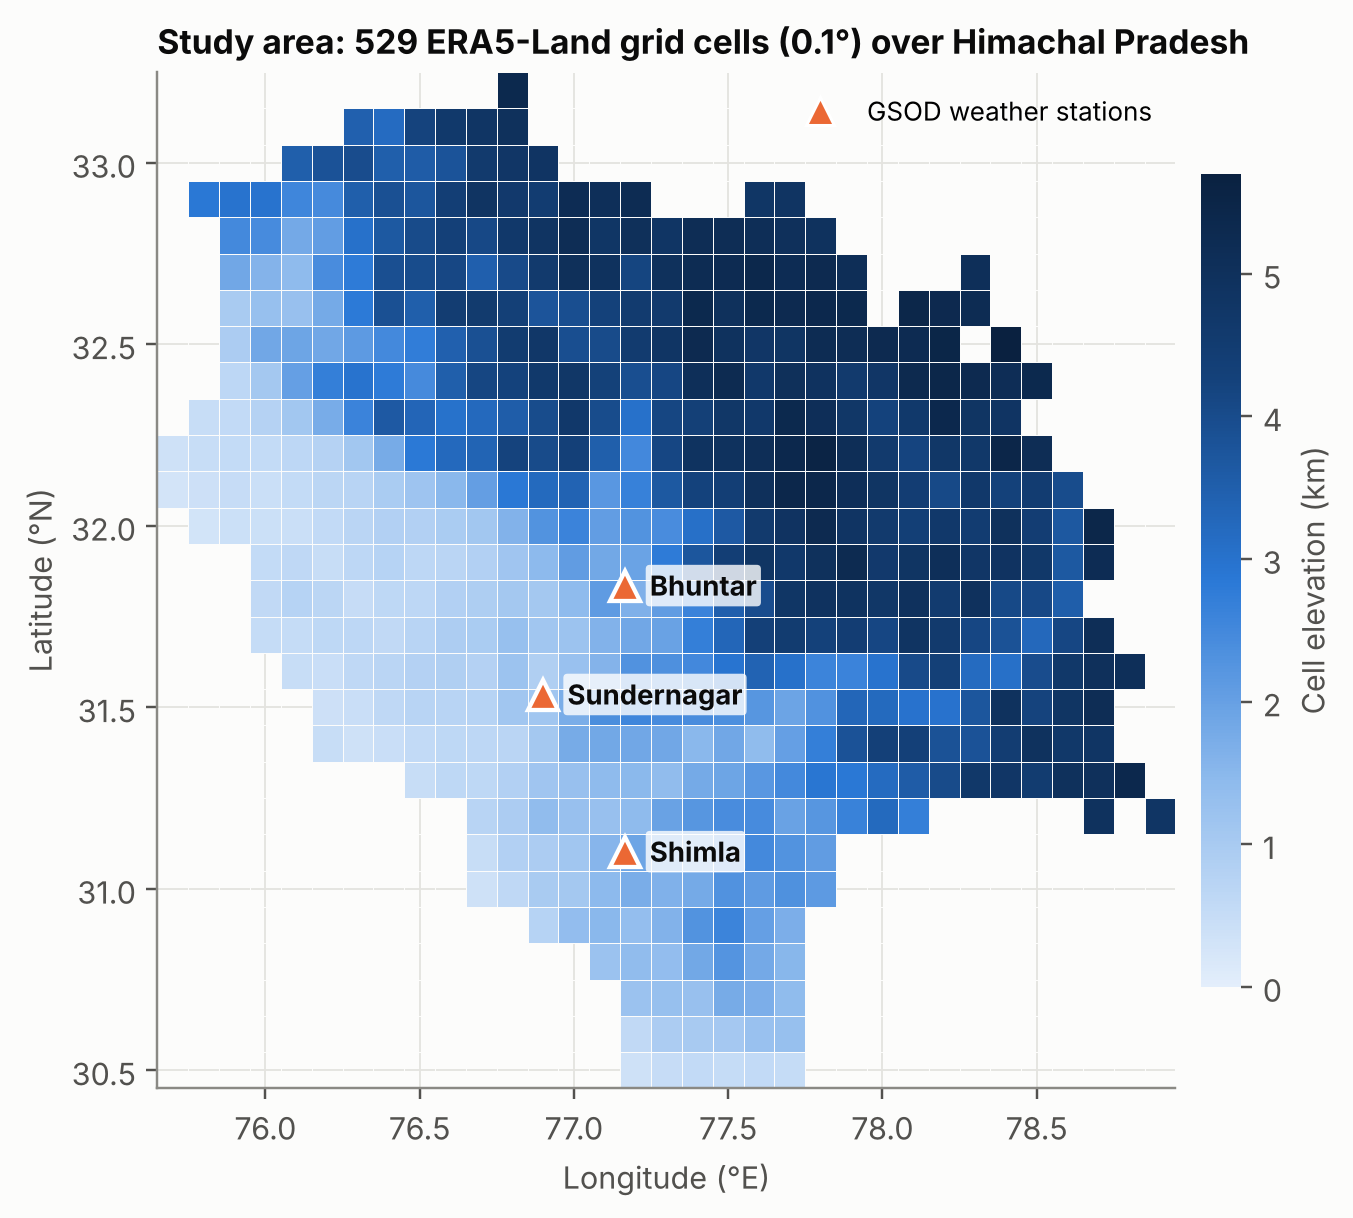
\includegraphics[width=0.62\textwidth]{fig_study_area.png}
\caption{The 529 cells coloured by elevation, and the three GSOD weather stations (kept for future checks).}
\end{figure}

\section{SRTM terrain}
SRTM (Shuttle Radar Topography Mission) is a map of ground height measured by radar from the Space Shuttle
\emph{Endeavour} in February 2000 (NASA). It gives a height every 30\,m. For each grid cell, the 30\,m heights were
averaged to give the cell's \textbf{mean elevation} (m), and the local slopes were averaged to give its \textbf{mean
slope} (degrees). These two numbers do not change with time; they tell the model whether a cell is a low valley or a
high, steep ridge.

\section{The variables and why each matters for heat}
\begin{table}[H]
\centering
\caption{Variables used. All except relative humidity come from ERA5-Land.}
\footnotesize
\begin{tabularx}{\textwidth}{>{\raggedright\arraybackslash}p{3.2cm}>{\raggedright\arraybackslash}p{1.4cm}>{\raggedright\arraybackslash}p{1.4cm}X}
\toprule
\textbf{Variable} & \textbf{Code} & \textbf{Unit} & \textbf{What it means and why it matters}\\
\midrule
Air temperature at 2\,m: daily max, min, mean & \texttt{t2m\_max}, \texttt{t2m\_min}, \texttt{t2m\_mean} & $^\circ$C
  & Temperature of the air at head height. The daily maximum defines the extreme day.\\
Dewpoint at 2\,m & \texttt{d2m} & $^\circ$C & The temperature at which the air would become saturated; higher means
  more moisture in the air.\\
Relative humidity & \texttt{rh} & \% & How close the air is to saturation, computed from temperature and dewpoint.
  Dry air heats faster.\\
Surface pressure & \texttt{sp} & hPa & Weight of the air above. Rising pressure usually means settled, clear, sunny
  weather.\\
Solar radiation down & \texttt{ssrd} & W\,m$^{-2}$ & Sunshine reaching the ground; the energy that heats it.\\
Soil water, top 7\,cm & \texttt{swvl1} & m$^3$\,m$^{-3}$ & Share of the soil volume that is water. Wet soil uses
  sunshine to evaporate water; dry soil turns it into heat.\\
Total precipitation & \texttt{tp} & mm & Rain (and melted snow) per day. Rain cools; dry spells come before heat.\\
Mean elevation, mean slope & \texttt{elev\_m}, \texttt{slope\_deg} & m, $^\circ$ & From SRTM. Temperature falls
  about 6.5\,$^\circ$C per km of height.\\
\bottomrule
\end{tabularx}
\end{table}

\textbf{Unit conversions done:} temperature K $\to$ $^\circ$C ($-273.15$), pressure Pa $\to$ hPa ($\div100$), rain
m $\to$ mm ($\times1000$), radiation J\,m$^{-2}$ per day $\to$ W\,m$^{-2}$ ($\div86{,}400$). Rain and radiation are
\emph{accumulated} in ERA5-Land: the value stamped at midnight of day $D+1$ is the total for day $D$, so they were moved
back one day.

\section{Seasons}
The India Meteorological Department (IMD) divides the year into four seasons, used throughout the project:
\begin{center}
\begin{tabular}{llc}
\toprule
\textbf{Season} & \textbf{Months} & \textbf{Days}\\
\midrule
Winter & December, January, February & about 90\\
Pre-monsoon & March, April, May & 92\\
Monsoon & June, July, August, September & 122\\
Post-monsoon & October, November & 61\\
\bottomrule
\end{tabular}
\end{center}

\begin{sayit}
``I used ERA5-Land, a reanalysis from ECMWF: a weather model corrected with real observations, giving gap-free daily
weather on a 9\,km grid. Inside Himachal that is 529 cells for 45 years. Height and slope of each cell come from NASA's
SRTM terrain map.''
\end{sayit}
